\chapter{\label{chap:spelunky}Spelunky}
Spelunky\footnote{http://www.spelunkyworld.com/original.html} é um jogo onde o
jogador incorpora um aventureiro que decide explorar uma caverna misteriosa. O
local contém tesouros, mas também está repleto de perigos. O objetivo principal
do jogador é explorar estas cavernas subterrâneas e coletar a maior quantia de
tesouros possível enquanto evita ser abatido pelos diversos inimigos e
armadilhas espalhadas pelo ambiente.

O jogo se enquadra no gênero \textit{platformer}, estilo de jogo que envolve
guiar um personagem através de plataformas suspensas e obstáculos para obter
progresso no jogo, e é fortemente inspirado em alguns dos elementos-chave do
gênero \textit{roguelike} -- tipo de jogos que se popularizou na década de 80
caracterizados por sua dificuldade, enfoque em exploração de ambientes e
narrativa fantasiosa --, como \textbf{geração procedural} e \textbf{morte
permanente} (Estes elementos são explicados em detalhe nas seções
\ref{section:spelunky-procgen} e \ref{section:spelunky-structure}). A Figura
\ref{fig:spelunky-gameplay} ilustra uma partida do jogo.

\begin{figure}[htb!]
\centering
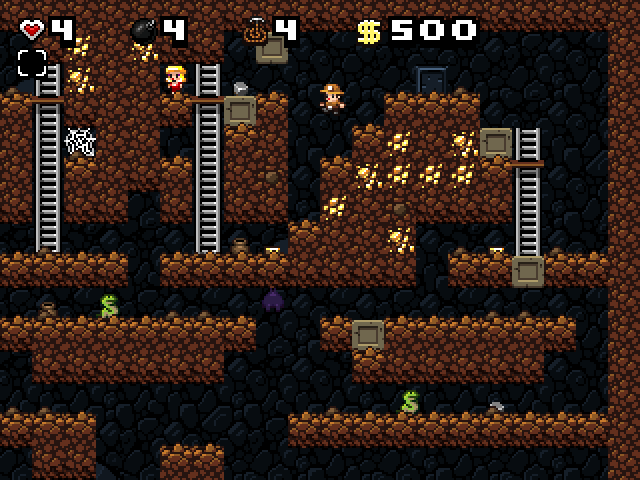
\includegraphics[width=.65\textwidth]{fig/spelunky-pc-screen.png}
\caption{\label{fig:spelunky-gameplay}Exemplo de partida de spelunky, mostrando
elementos do jogo como o jogador, a caverna, os inimigos, os tesouros, entre
outros.}
\end{figure}


%----------
\section{\label{section:spelunky-goals}Objetivos}
Apesar de o \textbf{objetivo principal} em Spelunky ser completar todos os
níveis, o jogo baseia a qualidade das partidas utilizando um sistema de
\textit{high scores}. Para tal, faz uso de uma série de métricas para
classificar os jogadores ao término de uma partida. Estas métricas são:

\begin{itemize}
	\item \textbf{Pontuação:} Mede a quantidade de tesouros obtidos pelo jogador
	no decorrer da partida. Existem diversos tipos de tesouros, como barras de
	ouro, pedras preciosas e estatuetas sagradas. Salvas as estatuetas sagradas,
	que devem ser carregadas até o fim do nível, o jogador precisa simplesmente
	tocar um tesouro para coletá-lo. Os tesouros se encontram espalhados pelo
	chão, dentro do terreno, dentro de baús ou são deixados por certos inimigos
	ao serem abatidos.

	\item \textbf{Tempo:} Mede o tempo para completar a partida. Começa a contar
	a partir do momento em que o jogador entra no primeiro nível e para de
	contar no fim do último nível. A contagem de tempo é interrompida durante as
	transições de nível e quando o jogador pausa a partida.

	\item \textbf{Abates:} Quantidade de inimigos abatidos pelo jogador durante
	a partida. Mortes acidentais de inimigos -- cair de um penhasco, acionar uma
	armadilha, etc. -- não aumentam este contador.

	\item \textbf{Salvamentos:} Quantidade de donzelas em perigo que foram
	resgatadas pelo jogador. Geralmente existe uma donzela em perigo por nível,
	mas existe a possibilidade -- mesmo que pequena -- de uma donzela não
	aparecer em alguns níveis. Para resgatar uma donzela, o jogador deve
	carregá-la com vida até a saída do nível.
\end{itemize}

Embora o jogo ofereça 4 métricas de classificação diferentes, a comunidade de
jogadores de Spelunky não mostra interesse significativo em atingir quantidades
elevadas de número de abates e número de salvamentos, se concentrando apenas em
atingir pontuações máximas e em concluir o jogo no menor tempo
possível\footnote{Comunidade de ranking de jogadores de Spelunky:
https://mosstier.com}. Pode-se concluir, portanto, que os \textbf{objetivos
secundários} mais importantes são a pontuação final e o tempo de partida. A
Figura \ref{fig:spelunky-scores} mostra um exemplo de pontuação final obtida.

\begin{figure}[htb!]
\centering
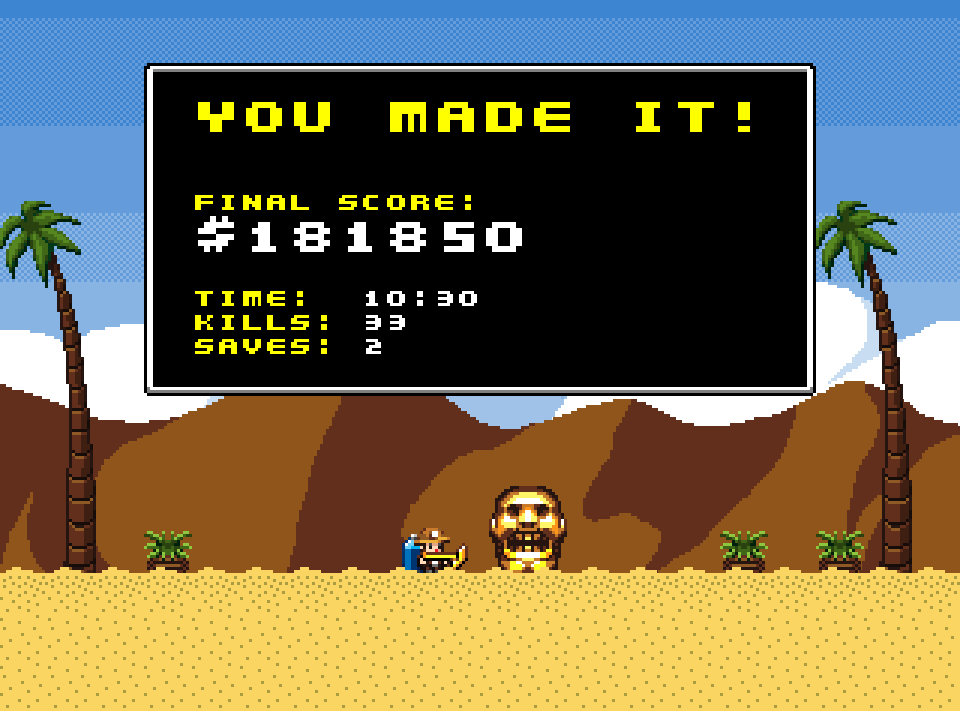
\includegraphics[width=.65\textwidth]{fig/spelunky-score.png}
\caption{\label{fig:spelunky-scores}Exemplo de pontuação final obtida ao fim de
uma partida de Spelunky.}
\end{figure}


%----------
\section{\label{section:spelunky-structure}Estrutura do jogo}
Uma partida de Spelunky é dividida em \textbf{níveis}, cada um sendo
representado por um mapa diferente. O jogador, ao entrar em um nível, é
posicionado na parte superior do mapa. Como não é informado ao jogador a posição
exata da saída, ele deve explorar o ambiente até encontrá-la. A saída sempre
está localizada em algum lugar na parte mais inferior do mapa. Ao utilizar a
saída, o jogador é enviado para o próximo nível e não pode retornar ao mapa que
acabou de completar.

O jogo é dividido em 4 \textbf{áreas} principais: \textbf{As Minas} (níveis 1 a
4), \textbf{A Selva} (níveis 5 a 8), \textbf{As Cavernas de Gelo} (níveis 9 a
12) e \textbf{O Templo} (níveis 13 a 16). Cada área possui um estilo de mapa e
aparência única. A dificuldade do jogo também aumenta gradativamente conforme o
jogador avança pelas áreas, principalmente porque os inimigos vão se tornando
cada vez mais fortes. O último nível do Templo é o \textbf{Covil de Olmec}. onde
o jogador deve enfrentar e derrotar \textbf{Olmec}. Após derrotar o inimigo
final, o explorador é recompensado com uma estatueta gigante feita de ouro e o
jogo termina.


\subsection{Atalhos}
É possível, ao iniciar uma partida, burlar este progresso entre áreas e ir
diretamente para as três ultimas áreas do jogo utilizando atalhos, criados pelo
personagem conhecido como \textbf{Homem do Túnel}. Para ter acesso a estes
atalhos, o jogador deve primeiramente auxiliar o Homem do Túnel a criá-los. O
personagem sempre aparece ao fim do último nível das primeiras três áreas do
jogo -- níveis 4, 8 e 12 --, se oferecendo para criar uma passagem secreta que
leva ao início da área que o jogador está prestes a chegar. Para criar a
passagem, o jogador deve ceder ao Homem do Túnel uma certa quantia de dinheiro.
O atalho da Selva, das Cavernas de Gelo e do Templo custam 100.000, 200.000 e
300.000, respectivamente.

Uma vez construídas, estas passagens são permanentes e podem ser acessadas ao
início de uma partida. Contudo, é importante ressaltar que, ao burlar etapas do
jogo, a pontuação do jogador não será contada para os \textit{high scores}.

\begin{mdframed}[backgroundcolor=green!20]
\begin{itemize}
    \item
		Colocar imagem do Homem do Túnel
\end{itemize}
\end{mdframed}


\subsection{Áreas Secretas}
Além das áreas principais, existem duas áreas secretas: \textbf{O Mercado Negro}
e \textbf{A Cidade de Ouro}. Estas áreas do jogo são fundamentais para se obter
equipamentos e grandes quantidadeds de tesouros, mas o jogador só obterá acesso
a elas se respeitar uma série de requisitos impostos pelo jogo. A Figura
\ref{fig:spelunky-secret-areas} exemplifica a aparência destas áreas secretas.

\begin{figure}[htb!]
\centering
	\begin{subfigure}[b]{0.4\textwidth}
		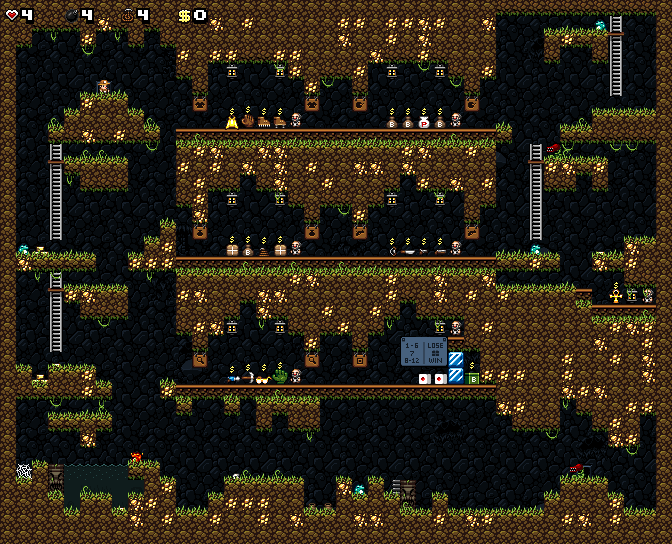
\includegraphics[width=\textwidth]{fig/spelunky-blackmarket.png}
		\caption{O Mercado Negro}
		\label{fig:spelunky-blackmarket}
	\end{subfigure}
	\begin{subfigure}[b]{0.4\textwidth}
		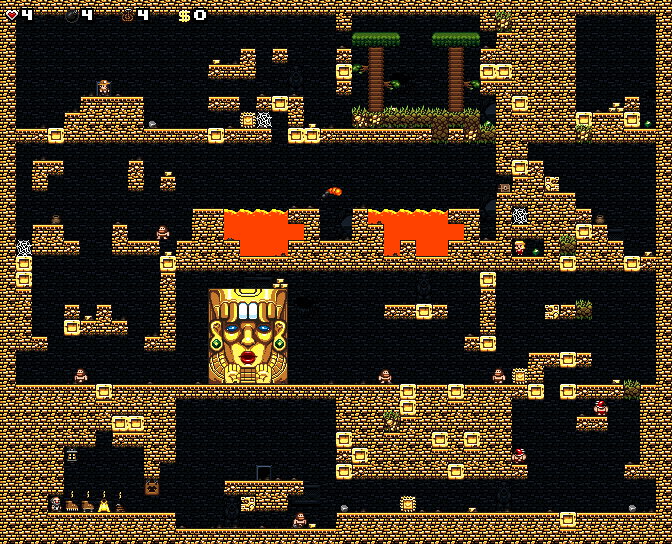
\includegraphics[width=\textwidth]{fig/spelunky-cityofgold.png}
		\caption{A Cidade de Ouro}
		\label{fig:spelunky-cityofgold}
	\end{subfigure}
	\caption{Exemplos das áreas secretas que podem ser acessadas pelo jogador em
	\textit{Spelunky}}
	\label{fig:spelunky-secret-areas}
\end{figure}


Para entrar no Mercado Negro, o jogador deve encontrar sua entrada -- que estará
oculta dentro do terreno do mapa -- enquanto explora a área da selva. O jogador
pode utilizar um item especial chamado \textbf{Udjat Eye} para ajudá-lo a
encontrar a entrada da área. O uso do item não é necessário, mas é aconselhável,
pois é quase impossível de localizar a entrada sem ele. Dentro do mercado negro,
o jogador encontrará vários comerciantes e terá a oportunidade de trocar seus
tesouros por equipamentos e itens diversos.

Entrar na Cidade de Ouro é muito mais complexo e é considerado um dos maiores
desafios do jogo, pois requer que o jogador colete uma série de artefatos
egípcios -- ilustrados na Figura \ref{fig:spelunky-artifacts} -- e execute uma
longa cadeia de ações ao longo da partida. A Cidade de Ouro é idêntica a um
nível do Templo, mas o terreno é feito de ouro maciço -- podendo ser destruído
com bombas -- e contém muito mais tesouros para coletar.  Além disso, o nível
contém uma estátua dourada gigante feita de ouro e pedras preciosas que pode ser
destruída pelo jogador. As etapas para entrar na Cidade de Ouro são:

\begin{enumerate}
	\item Coletar o \textbf{Udjat Eye}: O primeiro artefato se encontra dentro
	de um baú em algum nível da primeira área do jogo, as Minas. O jogador deve
	localizar a chave deste baú -- que se encontra no mesmo nível -- para poder
	abrí-lo. O Udjat Eye é capaz de encontrar a localização exata da entrada do
	Mercado Negro. O artefato pisca e brilha quanto mais próximo da entrada o
	jogador estiver, facilitando a localização da entrada.

	\item Coletar o \textbf{Ankh}: O segundo artefato se encontra no Mercado
	Negro e pode ser comprado (ou furtado) de um comerciante específico que
	vende somente este ítem. O Ankh oferece ao jogador uma segunda vida, caso
	venha a sucumbir.

	\item Coletar o \textbf{Hedjet}: O terceiro artefato pode ser obtido nas
	Cavernas de Gelo. Para obtê-lo, o jogador deve localizar um Moai\footnote{
	Estrutura monolítica com aparência humana. Os Moai foram esculpidos pelos
	Rapa Nui, habitantes nativos da Ilha de Páscoa.} e se morrer próximo a ele.
	O Ankh trará o jogador de volta a vida dentro do Moai e permitirá que o
	jogador colete o Hedjet.

	\item Coletar o \textbf{Cetro}: O quarto e último artefato podde ser obtido
	na última área do jogo, o Templo. O jogador deve encontrar e derrotar a
	Múmia, um dos inimigos mais fortes do jogo. Ao morrer, a múmia deixará o
	Cetro no chão. O Cetro é diferente dos outros itens porque, na verdade, é
	uma arma. Ele solta raios laser de cor rosa em formato de anel que perseguem
	e matam o inimigo mais próximo.

	\item Localizar a \textbf{Porta Dourada}: A última etapa do processo é
	encontrar a entrada da Cidade de Ouro, localizada em algum dos níveis do
	Templo. O jogador deve abandonar o Cetro e utilizá-lo como chave na Porta
	Dourada.
\end{enumerate}

\begin{figure}[htb!]
\centering

\includegraphics[width=.65\textwidth]{fig/spelunky-artifacts.png}
\caption{\label{fig:spelunky-artifacts}Os artefatos místicos de
\textit{Spelunky} necessários para acessar a Cidade de Ouro. Da esquerda para a
direita: o Udjat Eye, o Ankh, o Hedjet e o Cetro.}
\end{figure}

Não é necessário que o jogador acesse as duas áreas secretas do jogo durante uma
partida, mas as quatro áreas principais devem necessáriamente ser visitadas --
salvo quando o jogador fizer uso de um atalho, abrindo mão da validez de sua
pontuação. É importante ressaltar que o jogo conta com o conceito de
\textbf{morte permanente}, que faz com que o jogador, ao ter seus pontos de vida
esgotados, tenha que recomeçar o jogo desde seu início, perdendo todo o
progresso obtido até então.  A Figura \ref{fig:spelunky-run} ilustra a relação
entre as áreas e o progresso de uma partida de Spelunky.

\begin{figure}[htb!]
\centering
\begin{tikzpicture}[
    room/.style={
        regular polygon, regular polygon sides=4,
        draw=black, fill=white,
        text width=4.5em, text centered,
        minimum size=5mm,
        font=\small
    }
]
\matrix(rooms)[row sep=1cm, column sep=1cm]
{
    \node[room] (r1) {As Minas};            &
    \node[room] (r2) {A Selva};             &
    \node[room] (r3) {As Cavernas de Gelo}; &
    \node[room] (r4) {O Templo};            &

    \\
                                            &
    \node[room] (r5) {O Mercado Negro};     &
                                            &
    \node[room] (r6) {A Cidade de Ouro};    &
    \\
};
\draw[->,>=latex] (r1.east) -- (r2.west);
\draw[->,>=latex] (r2.east) -- (r3.west);
\draw[->,>=latex] (r3.east) -- (r4.west);

\draw[->,>=latex] ([xshift=-.5cm]r2.south) -- ([xshift=-.5cm]r5.north);
\draw[->,>=latex] ([xshift=.5cm]r5.north) -- ([xshift=.5cm]r2.south);

\draw[->,>=latex] ([xshift=-.5cm]r4.south) -- ([xshift=-.5cm]r6.north);
\draw[->,>=latex] ([xshift=.5cm]r6.north) -- ([xshift=.5cm]r4.south);
\end{tikzpicture}
\caption{\label{fig:spelunky-run}Relação entre as áreas de Spelunky durante uma
partida do jogo.}
\end{figure}

%----------
\section{\label{section:spelunky-controls}Controle do Personagem}
Os controles básicos em Spelunky são relativamente simples. Para se deslocar
pelo mapa, o jogador pode enviar comandos ao personagem para \textbf{caminhar},
\textbf{correr} e \textbf{pular}. O explorador também pode se \textbf{pendurar}
com as mãos na lateral de uma plataforma e subir e descer escadas. Como a
visibilidade do mapa é limitada a tela, o jogador pode \textbf{mover a câmera}
levemente na vertical ao \textbf{olhar para cima} ou se \textbf{agaixar},
aumentando sua visibilidade do ambiente. O explorador pode \textbf{utilizar
bombas e cordas} para auxiliar no deslocamento pelo nível. As bombas causam uma
explosão que elimina os inimigos e também desobstrui passagens. Já as cordas
permitem que o personagem atinja partes do mapa que não seriam acessíveis ao
pular, por estarem muito elevadas. Existe a possibilidade, também, de
\textbf{comprar itens} e \textbf{realizar apostas} com tesouros nas lojas dos
comerciantes.

A complexidade nos controles de Spelunky surge com a combinação de ações com
objetos, acessórios e equipamentos. O jogador pode \textbf{carregar um
item} em suas mãos e utilizá-lo quando desejar. O efeito depende do item
equipado atualmente. Por exemplo, se estiver carregando uma pedra, ele o
arremessará para longe. Se estiver segurando uma espingarda, ele realizará um
disparo. Os acessórios e equipamentos também modificam o funcionamento de ações.
Alguns acessórios podem fazer com que o personagem pule mais alto ou seja capaz
de se agarrar nas paredes. Portanto, é necessária atenção para os itens
coletados e equipados atualmente pelo explorador.


%----------
\section{\label{section:spelunky-procgen}Algoritmo de Geração Procedural de
Níveis}
Os níveis de Spelunky são gerados proceduralmente, ou seja, utiliza
um algoritmo capaz de gerar automáticamente os elementos que irão compor o
nível. Isto significa que não existe uma maneira de se memorizar estratégias
específicas de um mapa em Spelunky, pois ao início de cada partida o mapa é
gerado de maneira única e os tesouros, itens e obstáculos são dispostos de
maneira diferente, fazendo com que o jogador tenha que aprender a lidar com os
elementos do jogo de forma individual, combinar este conhecimento e estabelecer
uma estratégia para vencer seus obstáculos e ser bem sucedido.

O algoritmo de geração procedural de níveis de Spelunky é dividido em três
etapas: a \textbf{geração do caminho de solução}, a \textbf{geração de salas} e
a \textbf{disposição de entidades}.

\subsection{\label{section:spelunky-procgen-path}Geração do Caminho de Solução}
Cada nível em Spelunky é construído a partir de 16 \textbf{salas}, dispostas em
uma grade 4 por 4. Nesta etapa do algoritmo é escolhido o \textbf{caminho
solução} do nível, uma sequência de salas que formam um caminho desobstruído da
entrada até a saída. Primeiramente, o gerador escolhe uma das quatro salas da
parte superior para colocar a entrada do nível. Escolhido o local da entrada, o
algoritmo gera um caminho até a saída através de movimentos aleatórios para a
esquerda, para a direita e para baixo na grade de salas. Caso o gerador atinja
um dos extremos horizontais da grade, ele se desloca para baixo e inverte a
direção horizontal do movimento anterior. A saída do nível é colocada quando o
algoritmo chega na última linha da grade e tenta realizar um movimento para
baixo. Assim, a saída sempre se encontrará em uma das quatro salas da parte
inferior do mapa.

Todas as salas que fazem parte do caminho solução são transponíveis do início ao
fim sem o uso de bombas, cordas ou outros equipamentos. Além disso, sempre
possuem aberturas na esquerda e na direita. As salas em que o caminho realiza
uma descida possuem aberturas embaixo e as salas onde o caminho chega de uma
descida possuem aberturas em cima. Isto garante que haverá conectividade entre
todas as salas do caminho principal. Já as salas que não fazem parte do caminho
solução não possuem esta garantia, podendo ser completamente seladas e somente
acessíveis utilizando algum equipamento ou destruindo parte do terreno. Estas
salas fora do caminho solução também podem ser lojas, altares de sacrifício,
altares de ídolos dourados, entre outras. A Figura
\ref{fig:spelunky-procgen-path} exemplifica um resultado desta etapa do
algoritmo.

\begin{figure}[htb!]
\centering
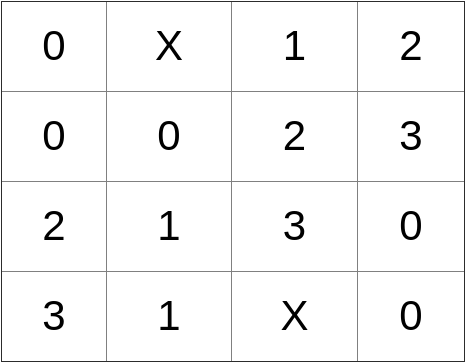
\includegraphics[width=.65\textwidth]{fig/spelunky-procgen-path.png}
\caption{\label{fig:spelunky-procgen-path}Exemplo de caminho solução gerado na
primeira etapa do algoritmo de geração procedural de níveis de Spelunky.}
\end{figure}

\begin{mdframed}[backgroundcolor=green!20]
\begin{itemize}
    \item
		Desenhar utilizando TikZ
\end{itemize}
\end{mdframed}

\subsection{\label{section:spelunky-procgen-rooms}Geração de Salas}
A próxima etapa do algoritmo é gerar separadamente as salas que irão compor o
nível. Para fazer isto, o gerador se baseia em \textit{layouts} de salas
pré-estabelecidos pelo desenvolvedor, sendo que cada tipo possui em torno de 6 a
12 \textbf{modelos}. Estes modelos são descritos através de sequências de
caracteres comuns. Uma sala em Spelunky é representada por uma grade 10 por 8 de
\textit{tiles}\footnote{Tipo de representação visual muito utilizada por jogos
2D para dispor os elementos de um jogo em forma de grade, onde cada elemento se
chama \textit{tile}.}, o que significa que cada modelo deve conter exatamente 80
caracteres. A Figura \ref{fig:spelunky-procgen-room-template} ilustra um exemplo
de modelo utilizado pelo gerador.

\begin{figure}[htb!]
\centering
\begin{tabular}{c c c c c c c c c c}
    0 & 0 & 0 & 0 & 0 & 0 & 0 & 0 & 1 & 1 \\
    0 & 0 & 6 & 0 & 0 & 0 & 0 & L & 0 & 4 \\
    0 & 0 & 0 & 0 & 0 & 0 & 0 & P & 1 & 1 \\
    0 & 0 & 0 & 0 & 0 & 0 & 0 & L & 1 & 1 \\
    0 & 0 & 0 & 0 & 0 & 0 & 0 & L & 1 & 1 \\
    0 & 0 & 0 & 0 & 0 & 0 & 0 & 0 & 1 & 1 \\
    0 & 0 & 0 & 0 & 0 & 0 & 0 & 0 & 1 & 1 \\
    1 & 1 & 1 & 1 & 1 & 1 & 1 & 1 & 1 & 1 \\
\end{tabular}
\caption{\label{fig:spelunky-procgen-room-template}Exemplo de modelo utilizado
para gerar uma sala de Spelunky.}
\end{figure}

Cada caractere possui um significado diferente, informando ao gerador que tipo
de \textit{tile} deve ser utilizado em sua posição. Eles podem ser
\textbf{estáticos} ou \textbf{probabilísticos}. Os estáticos sempre são
substituídos pelo seu \textit{tile} correspondente. Os caracteres "1" (bloco
sólido), "L" (escada) e "P" (escada com plataforma) são exemplos deste tipo. Já
os probabilísticos possuem uma chance de serem substituídos pelo seu
\textit{tile} correspondente ou por um espaço vazio. Os caracteres "2" (50\% de
chance de ocorrer um bloco sólido) e "4" (25\% de chance de ocorrer um bloco de
empurrar) são exemplos do segundo tipo.

Os caracteres "5" e "6" possuem uma característica especial. Eles não são
mapeados para um único \textit{tile}, e sim para um conjunto 5 por 3 de
\textit{tiles}, chamados de \textbf{obstáculos}. Estes conjuntos também utilizam
sequências de caracteres pré-definidos para descrever seu \textit{layout}.
Existem dois tipos de conjuntos, os aéreos e os terrestres. A diferença entre os
tipos de conjunto é simples: um conjunto terrestre deve ser colocado próximo ao
chão e um conjunto aéreo deve ser colocado no ar. Quando o gerador está
realizando a montagem da sala e detecta um caractere de obstáculo, ele realiza
uma substituição por um dos modelos disponíveis. A Figura
\ref{fig:spelunky-procgen-room-chunk} exemplifica um modelo de obstáculos.

\begin{figure}[htb!]
\centering
\begin{tabular}{c c c c c}
    0 & 1 & 1 & 1 & 0 \\
    0 & 2 & 2 & 2 & 0 \\
    0 & 0 & 0 & 0 & 0
\end{tabular}
\caption{\label{fig:spelunky-procgen-room-chunk}Exemplo de modelo de conjunto de
\textit{tiles} utilizado para gerar uma sala de Spelunky.}
\end{figure}

O uso destes conjuntos ajuda a aumentar a aleatoriedade dos \textit{layouts} das
salas, trazendo a sensação de uma variedade maior, mesmo que o número de modelos
de salas seja pequeno. O resultado da combinação do modelo da sala da
representada na Figura \ref{fig:spelunky-procgen-room-template} com o modelo de
obstáculos representado na Figura \ref{fig:spelunky-procgen-room-chunk} é
evidenciado na Figura \ref{fig:spelunky-procgen-room-combination}.

\begin{figure}[htb!]
\centering
\begin{tabular}{c c c c c c c c c c}
    0 & 0 & 0 & 0 & 0 & 0 & 0 & 0 & 1 & 1 \\
    0 & 0 & 0 & 1 & 1 & 1 & 0 & L & 0 & 4 \\
    0 & 0 & 0 & 2 & 2 & 2 & 0 & P & 1 & 1 \\
    0 & 0 & 0 & 0 & 0 & 0 & 0 & L & 1 & 1 \\
    0 & 0 & 0 & 0 & 0 & 0 & 0 & L & 1 & 1 \\
    0 & 0 & 0 & 0 & 0 & 0 & 0 & 0 & 1 & 1 \\
    0 & 0 & 0 & 0 & 0 & 0 & 0 & 0 & 1 & 1 \\
    1 & 1 & 1 & 1 & 1 & 1 & 1 & 1 & 1 & 1 \\
\end{tabular}
\caption{\label{fig:spelunky-procgen-room-combination}Exemplo de um modelo de
sala e um modelo de conjunto de \textit{tiles} utilizados para gerar uma sala de
Spelunky.}
\end{figure}

Com a descrição dos caracteres em mão, podemos realizar uma interpretação do
modelo ilustrado na Figura \ref{fig:spelunky-procgen-room-combination}. O modelo
descreve uma sala com chão, uma parede à direita, uma escada que leva a uma
pequena passagem, obstruída por um bloco de empurrar, e alguns blocos aéreos que
o jogador pode utilizar para se movimentar.

\subsection{\label{section:spelunky-procgen-entities}Disposição de Entidades}
A última etapa do algoritmo envolve a disposição dos inimigos, tesouros e
armadilhas. O algoritmo percorre todos os \textit{tiles} sólidos do nível a fim
de decidir se colocará uma entidade naquele local ou em suas proximidades.  Cada
tipo de entidade possui restrições diferentes:

\begin{description}
	\item[Inimigos]
	necessitam de espaços vazios acima ou abaixo do \textit{tile} sendo
	verificado atualmente. Inimigos não são colocados em locais muito apertados,
	dentro da água ou dentro da sala que contém a entrada do nível.

	\item[Tesouros]
	podem ser gerados acima de qualquer \textit{tile} sólido, mas a chance e
	valor do tesouro aumentam para locais apertados e em buracos no chão. Não
	são gerados perto da entrada e da saída.

	\item[Armadilhas]
	os requisitos variam muito de acordo com o tipo de armadilha, que podem ser
	espinhos, lança-flechas, pedregulhos, entre outros.
\end{description}

Cada entidade possui uma chance diferente de ocorrer a cada verificação, e as
probabilidades de ocorrência variam para cada área do jogo. Por exemplo, para
cada \textit{tile} na área das Cavernas, um morcego possui uma chance de 1.66\%
de ser gerado e um homem das cavernas possui uma chance de 0.12\% de ser gerado.
O algoritmo busca, através destas porcentagens, garantir que algumas entidades
apareçam mais frequentemente que outras, balanceando a dificuldade do jogo.

A Figura \ref{fig:spelunky-procgen-examples} exemplifica alguns níveis gerados
pelo algoritmo.

\begin{figure}[htb!]
\centering
	\begin{subfigure}[b]{0.4\textwidth}
		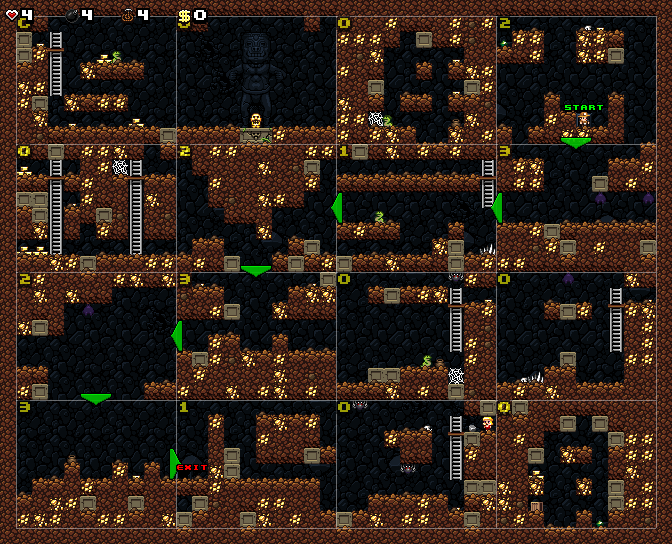
\includegraphics[width=\textwidth]{fig/spelunky-mines-example.png}
		\caption{As Minas}
		\label{fig:spelunky-mines-example}
	\end{subfigure}
	\begin{subfigure}[b]{0.4\textwidth}
		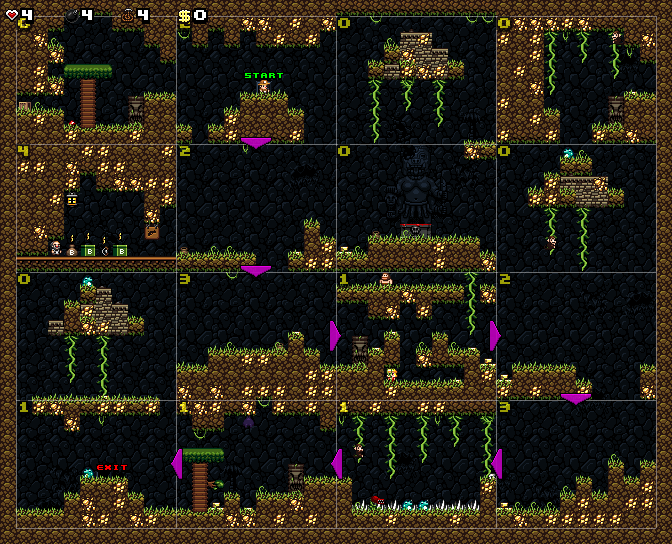
\includegraphics[width=\textwidth]{fig/spelunky-jungle-example.png}
		\caption{A Selva}
		\label{fig:spelunky-jungle-example}
	\end{subfigure}

	\begin{subfigure}[b]{0.4\textwidth}
		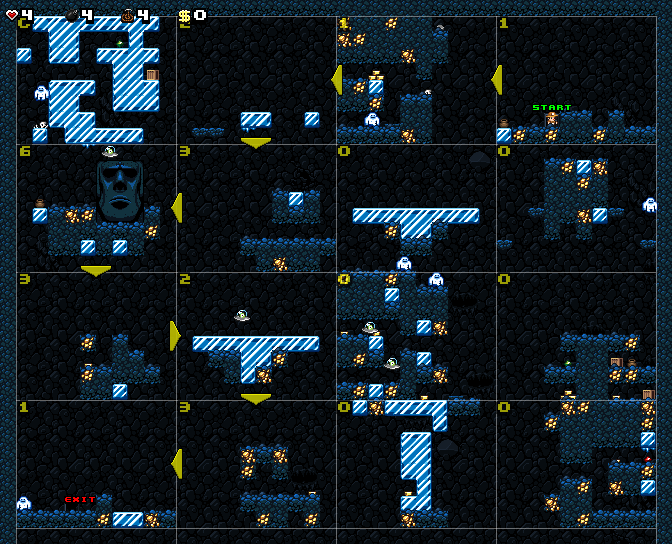
\includegraphics[width=\textwidth]{fig/spelunky-ice-example.png}
		\caption{As Cavernas de Gelo}
		\label{fig:spelunky-ice-example2}
	\end{subfigure}
	\begin{subfigure}[b]{0.4\textwidth}
		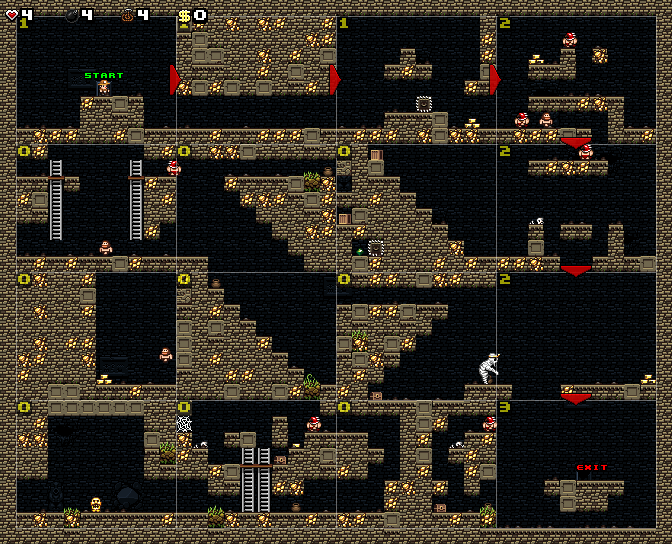
\includegraphics[width=\textwidth]{fig/spelunky-temple-example.png}
		\caption{O Templo}
		\label{fig:spelunky-temple-example}
	\end{subfigure}
	\caption{Exemplos do resultado final do algoritmo de geração de níves de
	\textit{Spelunky} para cada uma das áreas principais do jogo, com
	visualização da entrada, saída e caminho solução.}
	\label{fig:spelunky-procgen-examples}
\end{figure}


%----------
\section{\label{section:spelunky-obstacles}Obstáculos}
O universo de Spelunky é repleto de obstáculos, cujo único objetivo é impedir
que o jogador saia vivo de dentro das cavernas que está explorando. Estes
obstáculos podem ser \textbf{armadilhas} ou \textbf{monstros}. As armadilhas
são objetos projetados para punir invasores indesejados e os monstros são os
habitantes da caverna. Existem diversos tipos de armadilhas e monstros, e
alguns destes inclusive causam a morte instantânea do jogador. O anexo
\ref{section:spelunky-obstacles} apresenta a relação de monstros e
armadilhas, bem como uma breve descrição de seus comportamentos.

Além das armadilhas e monstros, o jogador também deve ter cuidado com os perigos
naturais presentes na caverna, como poços de lava e quedas de lugares muito
altos, pois também pode ser ferido por eles.


%----------
\section{\label{section:spelunky-items}Itens}
Em \textit{Spelunky}, existem diversos objetos com os quais o jogador pode
interagir para obter algum tipo de vantagem durante uma partida. Ao todo, são 43
itens diferentes, que são divididos nas seguintes categorias:

\begin{description}
	\item[Consumíveis]
	Objetos coletados pelo jogador que podem ser utilizados somente uma vez. Em
	alguns casos, o jogador pode carregar mais de um item consumível consigo.
	Alguns exemplo são as bombas, as cordas e o pára-quedas.

	\item[Acessórios]
	Equipamentos que, uma vez coletados pelo jogador, ficam disponíveis para uso
	durante toda a partida. Cada acessório oferece uma habilidade única que
	aumenta as chances de sobrevivência do explorador, e seus efeitos são
	manifestados ou passivamente -- sempre estão ativos -- ou através de uma
	ativação por parte do jogador. Alguns exemplos são o compasso, os sapatos de
	mola e a capa.

	\item[Armas]
	Equipamentos de combate de curto ou longo alcance carregados pelo explorador
	que o auxiliam a enfrentar os diversos monstros presentes na caverna. O
	jogador pode utilizar somente uma arma por vez, pois deve carregar a arma em
	suas mãos para utilizá-la. As armas não podem ser arremessadas pelo jogador.
	Alguns exemplos são o chicote, a espingarda e o arco.

	\item[Diversos]
	Objetos espalhados pela caverna que podem ser carregados e arremessados pelo
	jogador. Muitas vezes, servem como armas improvisadas, pois causam dano ao
	serem arremessadas e colidirem com algum inimigo. Também são utilizados para
	ativar armadilhas, impedindo que o jogador corra o risco de ativá-las sem
	querer. Alguns exemplos são as pedras, os vasos, as caixas e até mesmo
	corpos de inimigos abatidos. 
\end{description}

O anexo \ref{section:spelunky-obstacles} apresenta a relação de itens presentes
em \textit{Spelunky}, bem como uma breve descrição de seus comportamentos.


%----------
\section{\label{section:spelunky-dev}Desenvolvimento e Distribuição}

\begin{mdframed}[backgroundcolor=green!20]
\begin{itemize}
    \item
		Mencionar versão HD de \textit{Spelunky}
\end{itemize}
\end{mdframed}

O jogo foi desenvolvido por Derek Yu -- utilizando o motor de desenvolvimento de
jogos \textit{GameMaker} (Versão 8.0 Pro) -- e lançado gratuitamente para a
plataforma \textit{Windows} em dezembro de
2008\footnote{https://forums.tigsource.com/index.php?topic=4017}. No fim de
2009, o criador optou por liberar o código fonte do jogo, permitindo sua
distribuição não-comercial e
modificação\footnote{http://www.spelunkyworld.com/files/COPYING.txt}. A
liberação do código fonte de Spelunky pode ser considerada um marco muito
importante, pois permitiu que fossem criadas modificações para o jogo. Estas
modificações, que podem ser encontradas no fórum oficial da
\textit{Mossmouth}\footnote{http://mossmouth.com/forums/index.php} -- empresa
desenvolvedora de jogos criada por Derek Yu --, são correções de \textit{bugs},
mapas customizados ou até mesmo modos de jogo completamente diferentes do jogo
original. Pode-se dizer que dar esta liberdade para a comunidade do jogo é um
dos fatores que ajuda a manter sua base de jogadores e atraem novos jogadores
até hoje.

O motor GameMaker disponibiliza diversas ferramentas que facilitam o trabalho
do desenvolvedor. Contando com funcionalidades como editores de
\textit{scripts}\footnote{Código desenvolvido para o controle dos
comportamentos dos elementos do jogo.} e de \textit{sprites}\footnote{Elementos
visuais do jogo, tais como o personagem, o fundo, os inimigos. Representados
como uma ou mais imagens, permitindo que as mesmas sejam animadas.},
gerenciadores de eventos, entre
outras\footnote{http://sandbox.yoyogames.com/downloads/docs/gmaker80.pdf}, o
GameMaker oferece um ótimo suporte ao desenvolvedor para a criação de jogos. O
motor disponibiliza uma linguagem de programação própria para seus
\textit{scripts}, a \textit{GameMaker Language}, ou \textit{GML}.
